\chapter{Ocena użyteczności}

\begin{comment}
OCENA PRZYDATNOSCI UZYTECZNOSCI WALIDACJA
\end{comment}

System został dwukrotnie poddany walidacji. Pierwszy etap testów odbył się po ukończeniu implementacji pierwszego prototypu systemu. Drugi etap odbył się po ukończeniu drugiego prototypu, który poprawiał niedoskonałości odkryte podczas pierwszego etapu. 
Głównym celem przeprowadzonego procesu walidacji było sprawdzenie, czy implementowane rozwiązanie spełnia oczekiwania potencjalnych odbiorców. 

Do walidacji wytypowane zostały dwie funkcjonalności istotne dla działania systemu. Pierwszą z nich jest proces, który musi przejść każdy nowy użytkownik systemu, czyli tworzenie profilu zawodnika. Drugą z wybranych funkcjonalności jest poszukiwanie rywali oraz rzucanie im wyzwania. Jest to najważniejsza funkcja systemu zawierająca elementy interfejsu wymagające sprawdzenia użyteczności.


\section{Metodyka testów}

Testy odbyły się w formie badań moderowanych, czyli z udziałem osoby nadzorującej ich przebieg \cite{usstudywhatis}. Moderatorem w przypadku wszystkich badań był autor tej pracy. Rolą moderatora w przypadku takich badań jest obserwacja akcji podejmowanych przez osobę wykonującą zadania w systemie oraz sporządzanie notatek.

Do badań zostały wybrane osoby potencjalnie zainteresowane tematem, czyli osoby uprawiające sporty zespołowe. W celu zbadania użyteczności systemu dla różnych grup wiekowych zaproszono osoby w przedziale od 17 do 35 lat. Wśród ankietowanych były osoby profesjonalnie zajmujące się systemami webowymi jak również osoby spoza tej branży. Zgodnie z zaleceniami odnalezionymi w literaturze, w każdym z etapów badań wzięło udział pięciu respondentów \cite{usabilitystudy}.

Dla uczestników badania została przygotowana ankieta składająca się z trzech części. Pierwsza część była ankietą wstępną uzupełnianą przed badaniami. Zawierała ona krótkie wprowadzenie do systemu oraz pytania dotyczące wieku, profesji oraz umiejętności obsługi komputera osoby ankietowanej. Kolejne dwie części zawierały opisy zadań przygotowanych dla użytkowników oraz pytania kontrolne dotyczące intuicyjności poszczególnych procesów. 

Uczestnicy badania zostali poinformowani o tym, że obiektem badania jest interfejs systemu, a nie oni sami. Ze względu na obecność moderatora osoby uczestniczące w badaniu zostały poproszone o głośne myślenie oraz wyrażanie uwag. Moderator podczas badań na bieżąco notował istotne akcje podejmowane przez użytkowników oraz ich uwagi. Po wykonaniu zadań miała miejsce krótka dyskusja na temat zalet interfejsu, napotkanych problemów w obsłudze oraz potencjalnych usprawnień. Na podstawie notatek moderatora oraz ankiet zostały wyciągnięte wnioski dotyczące dalszego rozwoju interfejsu.

\section{Przebieg i wyniki badań}

W pierwszej kolejności do systemu zostały wprowadzone przykładowe (zmyślone) dane zawodników, drużyn oraz obiekty sportowe. Umożliwiło to wykonanie testów wymagających interakcji z innymi obiektami w systemie.

W poniższych sekcjach został opisany przebieg oraz wyniki badań poszczególnych funkcjonalności systemu. Szczegółowe wyniki w postaci złożonych ankiet oraz sporządzonych notatek można znaleźć na załączonej płycie.

\subsection{Tworzenie profilu zawodnika}

W ramach pierwszego zadania ankietowani zostali zalogowani na przygotowane konta użytkowników w systemie, a następnie poproszeni utworzenie profilu zawodnika. Krokami prowadzącymi do wykonania zadania było odnalezienie odpowiedniego formularza a następnie wypełnienie go. 

\subsubsection{Odnalezienie funkcjonalności}

Użytkownicy nie mieli problemów z odnalezieniem kreatora zawodnika. Dwie osoby zasugerowały, że formularz mógłby pokazywać się od razu po pierwszym logowaniu do systemu. Uwaga ta została uwzględniona w implementacji drugiego prototypu. 

\begin{figure}[H]
\centering
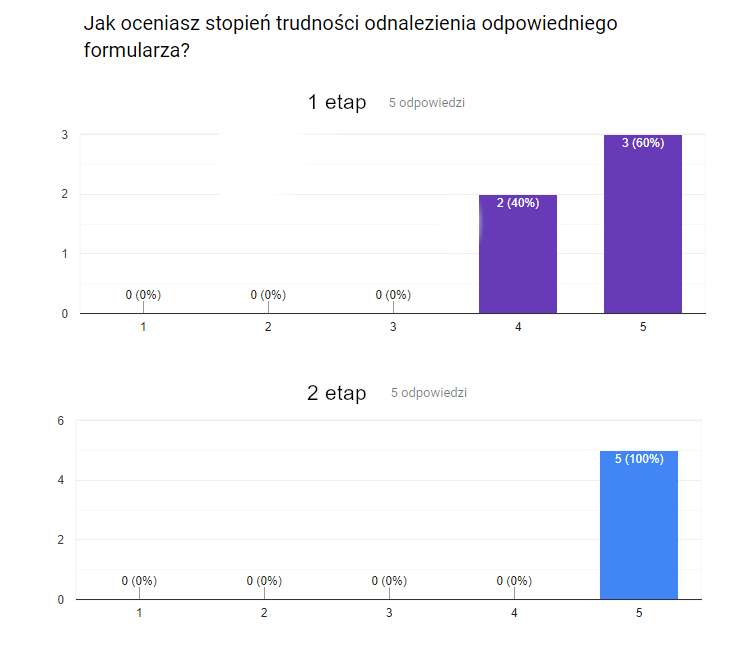
\includegraphics[width=0.8\linewidth]{07-walidacja/rys/survey-create-player.png}
\caption{Zestawienie ocen trudności odnalezienia formularza tworzenia zawodnika po pierwszym etapie badań (1 - bardzo trudne, 5 - bardzo łatwe)}
\label{fig:view-player-skill}
\end{figure}


\subsubsection{Nawigacja po formularzu}

Nawigacja po formularzu składającym się z paru kroków nie sprawiła żadnych problemów respondentom.

\subsubsection{Deklaracja poziomu umiejętności}

Krok polegający na deklaracji poziomu umiejętności również nie stanowił żadnych trudności. Każdy z ankietowanych był w stanie czytając opisy poszczególnych profili umiejętności dopasować się do jednego z nich. Dokonywanie wyborów poprzez przesunięcie suwaków było w pełni intuicyjne.
  
  \begin{comment}
\begin{figure}[H]
\centering
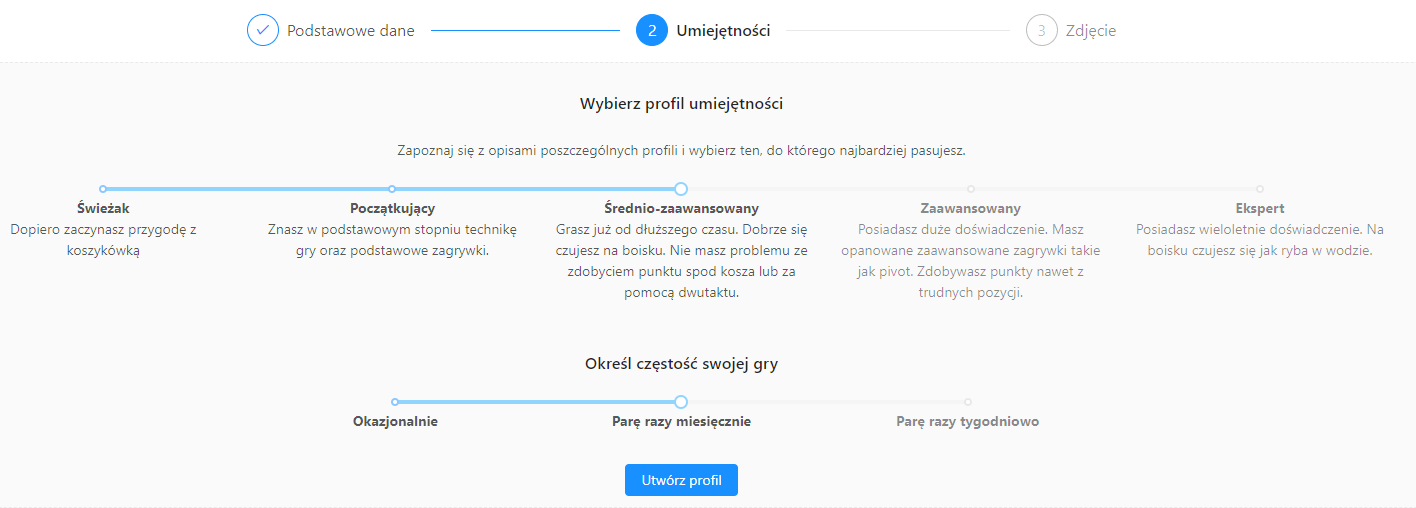
\includegraphics[width=\linewidth]{07-walidacja/rys/p_skill.PNG}
\caption{Widok po zalogowaniu się kapitana do systemu}
\label{fig:view-player-skill}
\end{figure}
\end{comment}

\subsection{Szukanie przeciwników i rzucanie wyzwania}

Drugie zadanie miało na celu sprawdzenie intuicyjności poszukiwania przeciwników oraz tworzenia wyzwania. Respondenci zostali zalogowani na przygotowane wcześniej konto kapitana jednej z drużyn i poproszeni o odnalezienie przeciwników o podobnym wieku w okolicy oraz rzucenie im wyzwania.

\subsubsection{Odnalezienie funkcjonalności}

Respondenci używający pierwszego prototypu odnaleźli odpowiedni formularz, jednak dla niektórych wymagało to trochę czasu. W drugim prototypie odnośnik umieszczono w centrum strony społeczności widocznej po zalogowaniu do systemu.

\begin{figure}[H]
\centering
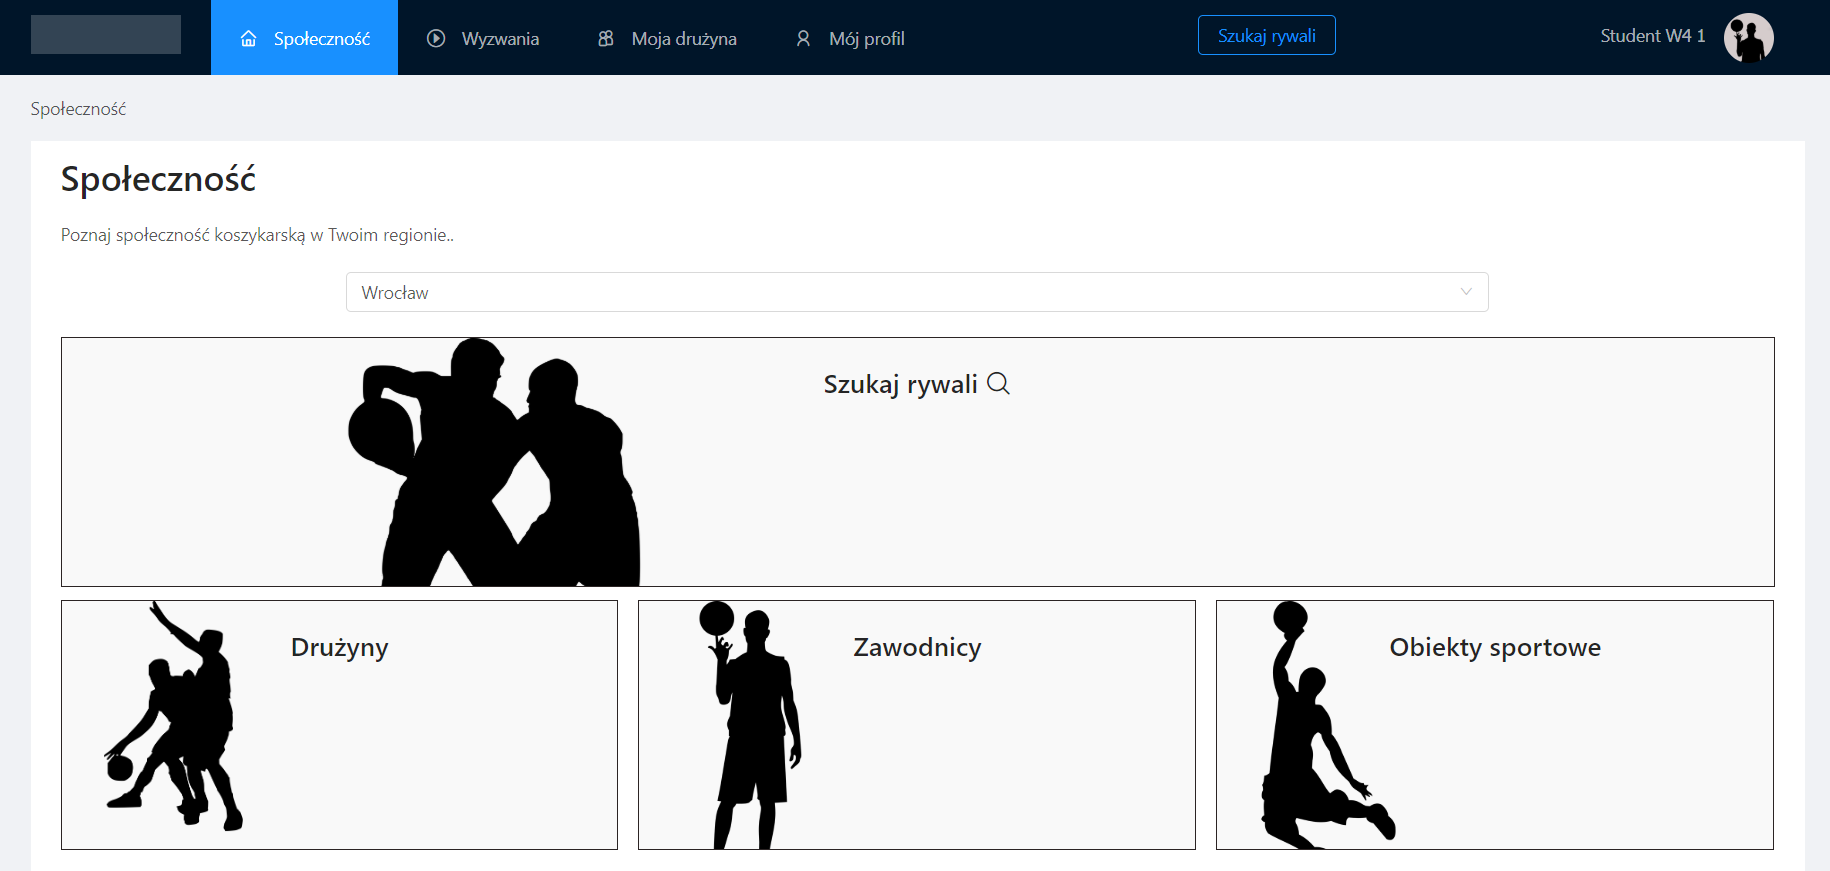
\includegraphics[width=\linewidth]{07-walidacja/rys/spolecznosc.PNG}
\caption{Widok po zalogowaniu się kapitana do systemu}
\label{fig:view-player-skill}
\end{figure}

\subsubsection{Deklaracja preferencji wyszukiwania}

Deklaracja preferencji odnośnie rywali okazała się być problematyczna dla części użytkowników. Zaproponowany w ramach pierwszego prototypu podział procentowy wprowadzał użytkowników w błąd. Z punktu widzenia algorytmu im bardziej znaczące jest dane kryterium tym większą wartość (wagę) powinno ono otrzymać. Użytkownicy jednak wartość 0\% utożsamiali z~brakiem różnicy a więc dobrym dopasowaniem. Z tego względu niektórzy respondenci ustawili suwaki odwrotnie niż było to wskazane. Interfejs przedstawiono na rysunku \ref{fig:suwaki-bef}

Dużą część uwagi podczas przygotowywania drugiego prototypu poświęcono poprawie intuicyjności tej funkcjonalności. W pierwszej kolejności przygotowano makietę nowego wyglądu i opisu funkcjonalności, która została przedstawiona respondentom i spotkała się z ich aprobatą. Następnie planowane zmiany zostały zaimplementowane i zweryfikowane podczas testów drugiego prototypu. Głównym usprawnieniem było zrezygnowanie z wartości procentowych na rzecz abstrakcji - punktów preferencji. Dodatkowo dodano symbole graficzne, dokładniejsze opisy poszczególnych wyborów oraz panel z pomocą odnośnie rozdzielania punktów preferencji. Interfejs po zmianach przedstawiono na rysunku \ref{fig:suwaki-aft}. 


\begin{figure}[H]
\centering
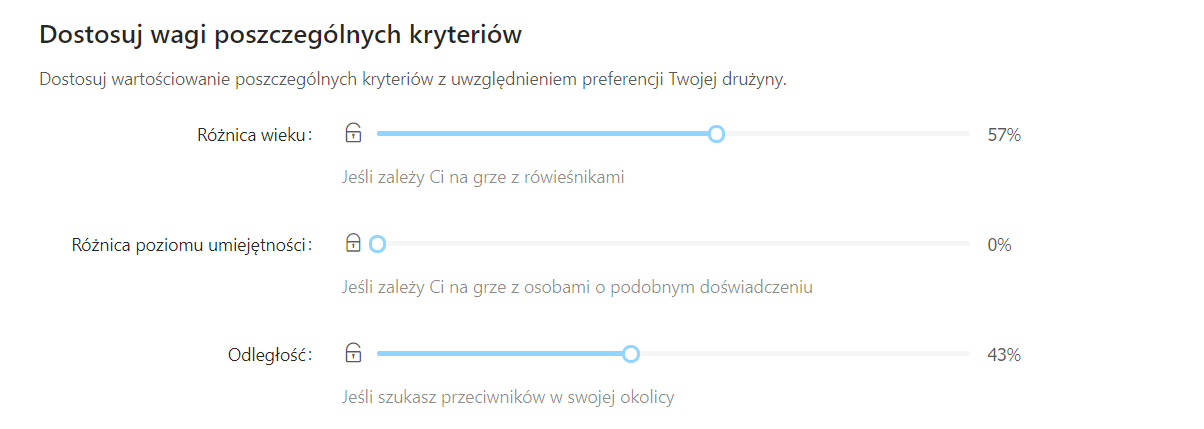
\includegraphics[width=\linewidth]{07-walidacja/rys/suwaki_before_close.PNG}
\caption{Formularz deklaracji preferencji przed zmianami - I prototyp}
\label{fig:suwaki-bef}
\end{figure}


\begin{figure}[H]
\centering
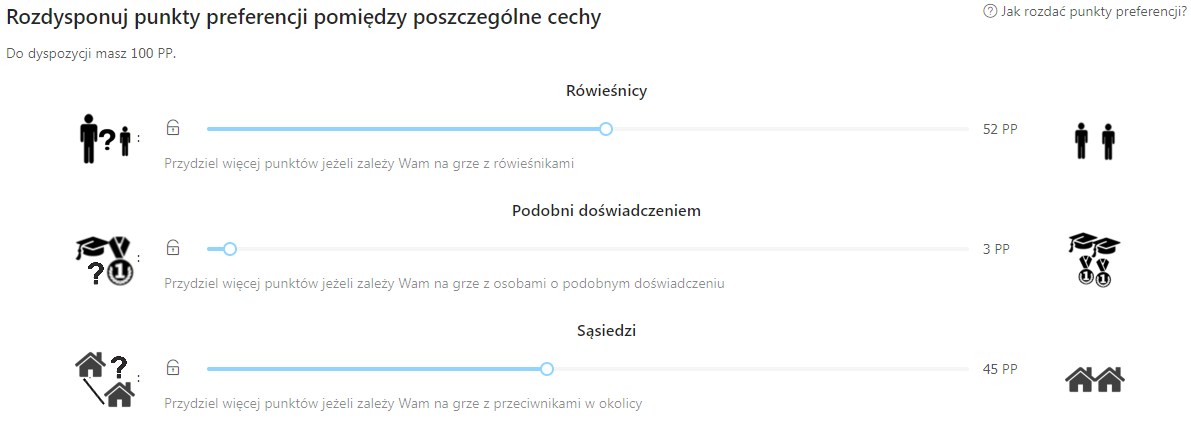
\includegraphics[width=\linewidth]{07-walidacja/rys/suwaki_after_close.PNG}
\caption{Formularz deklaracji preferencji po zmianach - II prototyp}
\label{fig:suwaki-aft}
\end{figure}

Wprowadzone usprawnienia przełożyły się na znaczne lepsze zrozumienie funkcjonalności przez respondentów. Rysunek \ref{fig:survey-suwaki} przedstawia zestawienie odpowiedzi osób ankietowanych przed oraz po wdrożeniu zmian.

\begin{figure}[H]
\centering
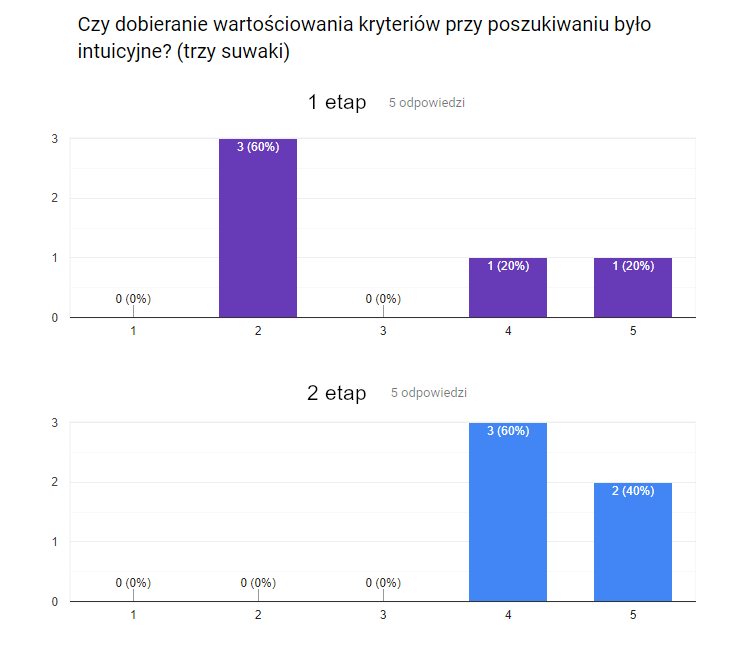
\includegraphics[width=\linewidth]{07-walidacja/rys/survey-search.png}
\caption{Zestawienie ocen intuicyjności deklaracji preferencji wyszukiwania (1 - nie intuicyjne, 5 - w pełni intuicyjne)}
\label{fig:survey-suwaki}
\end{figure}

\begin{comment}
\begin{figure}[H]
\centering
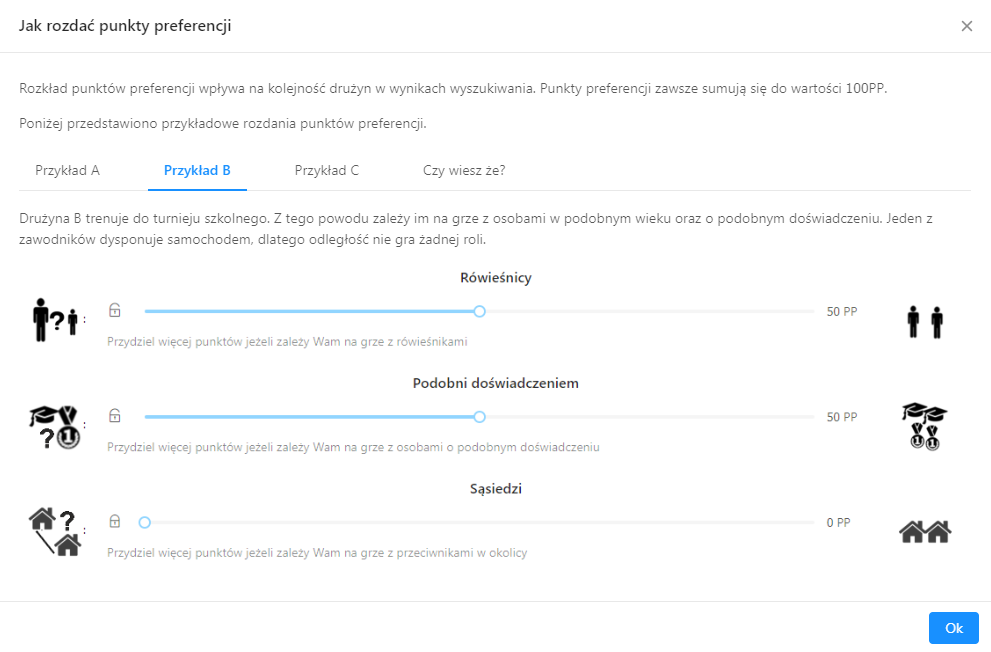
\includegraphics[width=\linewidth]{07-walidacja/rys/help.PNG}
\caption{Aaaaaa}
\label{fig:suwaki-help}
\end{figure}
\end{comment}

\subsubsection{Wyniki wyszukiwania oraz rzucanie wyzwania}

Sposób przedstawienia wyników wyszukiwania - proponowanych rywali okazał się być bardzo przystępny dla użytkowników. Respondenci byli w stanie na podstawie dostarczonych informacji wnioskować na temat dopasowania poszczególnych drużyn, a następnie rzucić wyzwanie jednej z nich. Proponowanie wstępnych ofert miejsca oraz czasu spotkania było zrozumiałe. W ramach tej części funkcjonalności w drugim prototypie zostały wprowadzone jedynie drobne zmiany. 
